\scanpage{44}
% archive foliation: 43
b) Si $u\in\operatorname{End}_K(\mathcal M)$, alors on définit
\[
\bar e_u:\overline G_{aK}\longrightarrow\unsure{\operatorname{Aut}|\operatorname{End}}_K(\mathcal M)
\]
\[
\bar e_u(\lambda)=\exp(\lambda u)
\]
\uline{NB} La question se pose encore si $u\longmapsto\bar e_u$ et $u\longrightarrow e_u$ sont des \uline{bij.}
\margin{?}
\[
\begin{aligned}
\operatorname{End}_K(\mathcal M)&\longrightarrow\operatorname{Hom}_{\mathrm{gr}}(\overline G_{aK},\operatorname{Aut}_K(\mathcal M))\\
N(\operatorname{End}_K(\mathcal M))&\longrightarrow\operatorname{Hom}_{\mathrm{gr}}(G_{aK},\operatorname{Aut}_K(\mathcal M))
\end{aligned}
\]
Extension aux \deleted{\unsure{f}} algèbres symétriques, tensorielles, \unsure{extérieures} ---

\figure{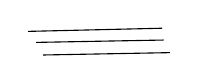
\begin{tikzpicture}[x=1cm,y=1cm]
\draw (0,0.30)--(1.7,0.34);
\draw (0.10,0.16)--(1.72,0.19);
\draw (0.19,0)--(1.80,0.03);
\end{tikzpicture}}
\deleted{\unsure{II}}

\uline{Globalisation} \deleted{\unsure{S|Soit}} $X$ schéma de car 0,

$\Theta$ \unsure{la|une} dérivation de $\underline O_X$, supposons $\Theta$ loc nilpotent. Alors $\exp\Theta$ est un autom de $\underline O_X$ qui induit l'identité sur $\underline O_{X_{\mathrm{réd}}}=\underline O_X/N\underline O_X$, et correspond à un autom de $X$ : que nous désignerons par $E_\Theta$. Si $\unsure{X}$ est sur $S$ et $\Theta$ est une $S$-dérivation, $E_\Theta$ est un $S$-autom. On a
\[
\left\{\begin{aligned}
E_0&=\operatorname{id}\\
E_{\Theta+\Theta'}&=E_\Theta+E_{\Theta'}\qquad\text{si }[\Theta\Theta']=0
\end{aligned}\right.
\]
